\documentclass[10pt,a4paper]{ltjsarticle}

\usepackage{graphicx}
\usepackage{amsmath,booktabs,subfig}
\usepackage{pifont}
\usepackage{url}
\usepackage{cite}

\usepackage{siunitx}
\usepackage{float}
\usepackage{tikz}
\usetikzlibrary{shadows}
\usetikzlibrary{calc}
\usepackage{circuitikz}

\usepackage{tcolorbox}

\usepackage{luatexja-fontspec}
%\setmainfont[Ligatures=TeX]{TeXGyreTermes}
%\setsansfont[Ligatures=TeX]{TeXGyreHeros}
\setmainfont{TimesNewRoman}
\setsansfont{Arial}
\defaultjfontfeatures{Scale=1.0}
\setmainjfont[BoldFont=IPAexGothic]{IPAexMincho}
%\setmainjfont[BoldFont=HiraMinProN-W6]{HiraMinProN-W3}
%\setmainjfont[BoldFont=IPAexGothic]{KozMinPr6N-Light}
%\setmainjfont[BoldFont=IPAexGothic]{MS-PMincho}
\setsansjfont{IPAexGothic}
%\setsansjfont{MS-PGothic}
%\setsansjfont[BoldFont=HiraginoSans-W8]{HiraginoSans-W4}

\begin{document}
\title{シンクロトロン振動のいろは}
\author{吉本伸一}
\maketitle
\tableofcontents
\clearpage

\section{はじめに}
蓄積リングでは,ビームに対して横方向(水平,垂直方向)へは4極磁石による収束力、縦方向(到着時間のずれ―エネルギー空間)へは高周波加速による収束力を発生させて、それぞれの方向へのポテンシャルを作り出し、ビームをその平衡点に閉じ込めている。横方向の振動をベータトロン振動、縦方向の振動をシンクロトロン振動とよぶ。


\section{高周波による繰り返し加速}
静電場を用いて荷電粒子を加速する場合、同じ加速電場を使って何度も繰り返し加速する事はできない。例えば図~\ref{dc_acc}のように磁場を使って荷電粒子を曲げ、何度も同じ電極を通過させた場合を考えてみよう。粒子は電極を通る時加速されるが、電極の外では逆に減速され加速した分が相殺されてしまう。このように、静電場を使って繰り返し加速はできないため、繰り返し加速を行う場合は、高周波電場を使うことになる。ただし、この図のように単純に平行平板の電極に高周波電圧を加えただけでは、静電場の時と同じように電極外で粒子が原則されてしまう場合がある。そこで、電磁場が外部に漏れないよう導体の壁によって囲まれた高周波加速空洞を使って繰り返し加速を行うことになる。

\begin{figure}[hbt]
  \begin{center}
    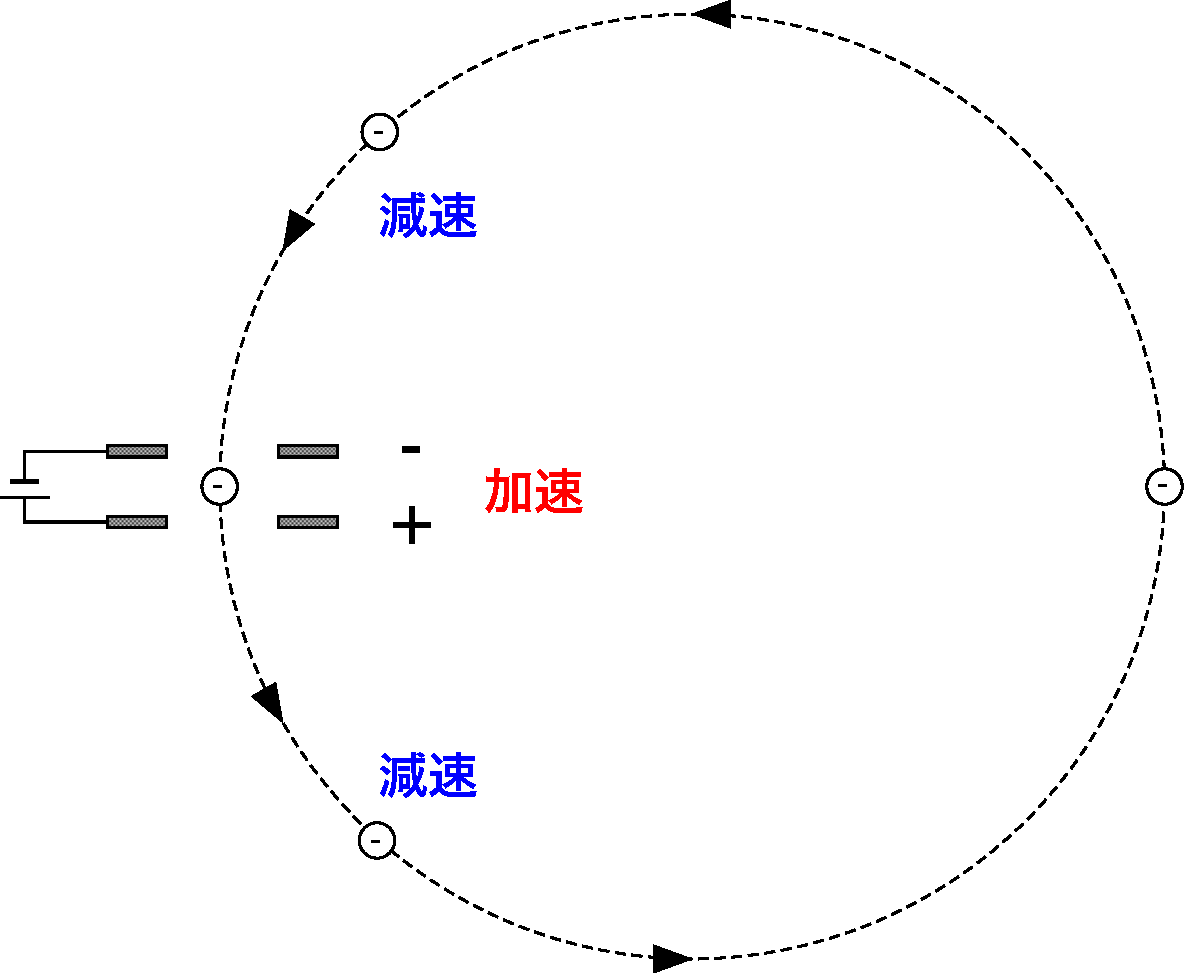
\includegraphics[width=10cm,clip]{dc_acc.pdf}
    \caption{静電場による繰り返し加速}
   \label{dc_acc}
  \end{center}
\end{figure}

\section{高周波加速空洞の基礎の基礎}
図~\ref{cavity1}はインダクタンス$L$とキャパシタンス$C$のよく知られた共振回路であり、この回路の共振周波数は、

\begin{equation}
  \omega = \frac{1}{\sqrt{LC}}
  \label{LC}
\end{equation}

で与えられる。いま、共振周波数が高いとき、(\ref{LC})より$L$と$C$は小さな値でもよく、極端な話、コイルの部分を引き伸ばして一本の線にした図~\ref{cavity2}のような回路でも共振回路として動作する。

\begin{figure}[hbt]
  \begin{center}
    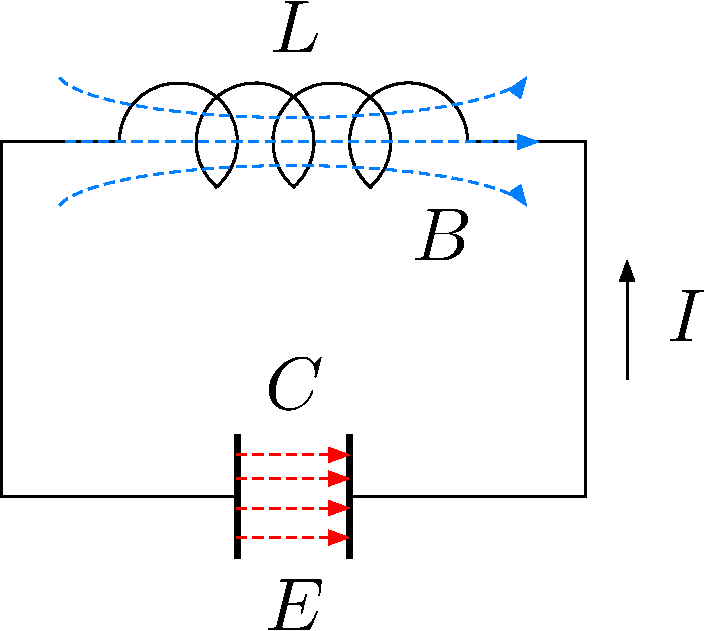
\includegraphics[width=8cm,clip]{cavity1.pdf}
    \caption{$LC$共振回路}
   \label{cavity1}
  \end{center}
\end{figure}

次に、この回路を$z$軸の周りに回転させると図~\ref{cavity3}のような金属の壁で囲まれたものが出来上がる。これも同様に共振回路として働き、空洞共振器と呼ばれる。空洞内では図に示すように。磁場は動径方向を周り、電場はギャップ部分に集中している。このギャップ部分に生じた高周波電場を使って荷電粒子を加速する装置が高周波加速空洞と言うことになる。

\begin{figure}[hbt]
  \begin{center}
    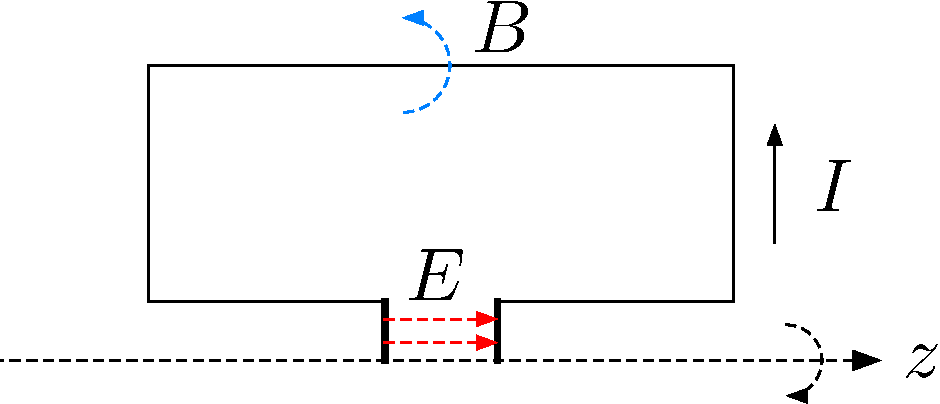
\includegraphics[width=8cm,clip]{cavity2.pdf}
    \caption{$LC$共振回路}
   \label{cavity2}
  \end{center}
\end{figure}

\begin{figure}[hbt]
  \begin{center}
    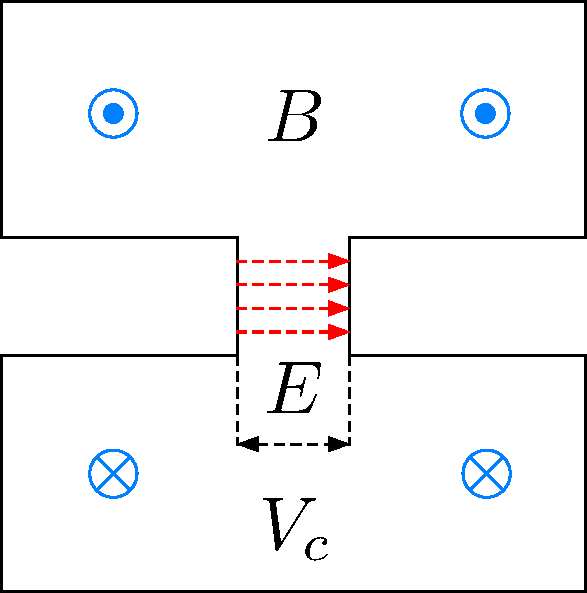
\includegraphics[width=6cm,clip]{cavity3.pdf}
    \caption{高周波加速空洞}
   \label{cavity3}
  \end{center}
\end{figure}

加速空洞の内面では、動径方向に走る磁場によって高周波電流が流れるので、空洞内面が持つ抵抗によって電力を損失する。したがって、共振状態を維持するためには外部より電力を供給する必要がある。いま、空洞の加速電圧を$V_{c}$、この電圧を維持するために必要な電力を$P_{c}$とすると、
%
\begin{equation}
  R_{sh} \equiv \frac{V_{c}^2}{P_{c}}
  \label{sh}
\end{equation}
%
で定義される量をシャントインピーダンスといい、空洞の特性を表す重要なパラメータの一つである。また、空洞内に蓄えられる電磁場のエネルギー$U$と空洞内の損失$P_{c}$を用いて、
%
\begin{equation}
  Q = \frac{\omega U}{P_{c}}
  \label{q_val}
\end{equation}
%
で表される量を空洞の$Q$値といい、これも空洞の特性を表す重要なパラメータとなっている。

\begin{tcolorbox}[title=\textgt{ARESとSCCの空洞損失}]
  ARESの場合、$Q_{0}=1.33\times10^5$、$R_{sh}=1.7\,\mathrm{M}\Omega$で、空洞一台当たりの加速電圧を$V_{c}=0.5\,\mathrm{MV}$とすると、
%
\begin{equation*}
  P_{c} = \frac{V_{c}^2}{R_{sh}}=147\,\mathrm{kW}
\end{equation*}

一方SCCの場合、$Q_{0}=1\times10^9$、$R_{sh}=93\times 10^3\,\mathrm{M}\Omega$で、空洞一台当たりの加速電圧を$V_{c}=1.5\,\mathrm{MV}$とすると、
%
\begin{equation*}
  P_{c} = \frac{V_{c}^2}{R_{sh}}=24\,\mathrm{W}
\end{equation*}
%
となり、SCCの方が圧倒的に損失が少ない。(流石超電導!)
\end{tcolorbox}

\section{同期粒子 (synchronous particle)}
高エネルギーの荷電粒子が磁場によって曲げられる時、その進行方向に向かって電磁波を放射してエネルギーを失う。この現象のことをシンクロトロン放射と呼び、放射された電磁波を放射光という。SuperKEKB, PF, PF-ARのような電子(陽電子)貯蔵リングでは、偏向電磁石で曲げられた電子(陽電子)がシンクロトロン放射によってエネルギーを失い、加速空洞内の高周波電場によって補填される。空洞の加速電圧は周期的に変化しており、そのピーク加速電圧$V_c$とRF周波数$f_{RF}$(もしくは$\omega_{RF}$)を用いて、
%
\begin{equation}
  V(t) = V_c\sin\left(2\pi f_{RF} t\right)=V_c\sin(\omega_{RF} t)
  \label{vc}
\end{equation}
%
と表すことができる。この式はまた、
%
\begin{equation}
  \phi(t) = 2\pi f_{RF} t=\omega_{RF} t
  \label{phase}
\end{equation}
%
を用いて。位相\phi の関数として、
%
\begin{equation}
  V\left(\phi\right) = V_c\sin(\phi)
  \label{eq7}
\end{equation}
%
と表すこともできる。粒子がリング一周する間に失うエネルギーを$U_0$を加速空洞で補うためには、
%
\begin{equation}
  U_0=e V\left(\phi_s\right)=e V_c \sin\phi_s
  \label{eq8}
\end{equation}
%
を満たすような位相$\phi_s$で空洞を通過する必要がある。この時、(\ref{eq7})に$e$を掛け、加速電圧と$U_0$の関係をプロットすると図~\ref{cavity_vol}のようになる。この図を見ると、(\ref{eq8})を満たすような位相は、加速電場の一周期の間に二回現れることがわかる。

\begin{figure}[hbt]
  \begin{center}
    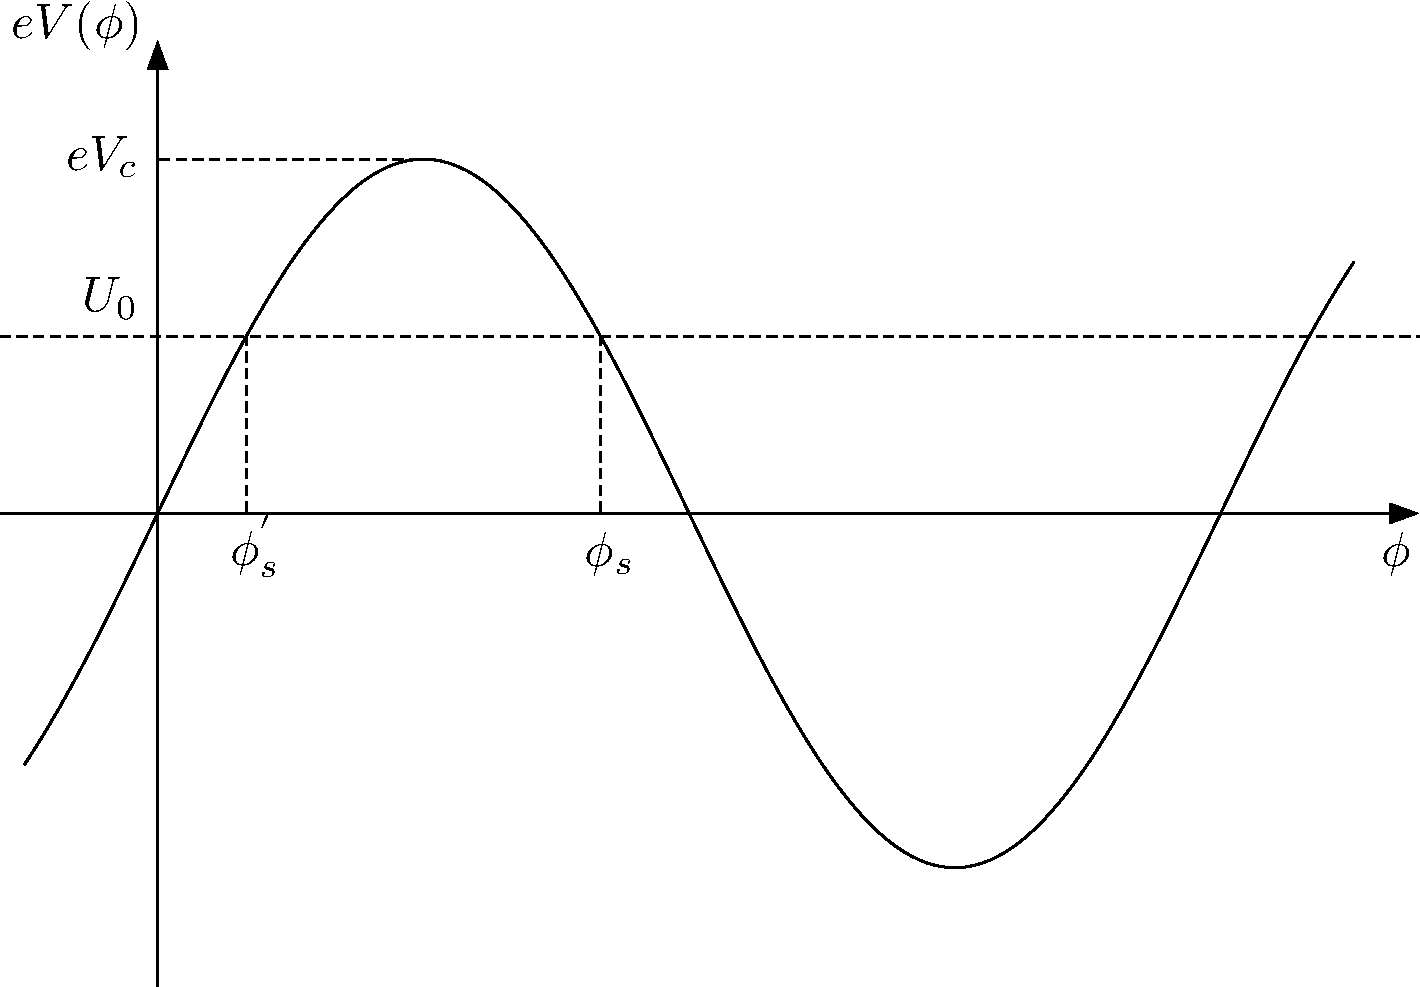
\includegraphics[width=12cm,clip]{cavity_vol.pdf}
    \caption{加速電圧と$U_0$の関係}
   \label{cavity_vol}
  \end{center}
\end{figure}

ある粒子が位相$\phi_s$で空洞に入った場合、この粒子がリングを一周して空洞に戻ってきたとき、再び同じ位相で空洞に入ると、エネルギーの収支のバランスが保たれ、その粒子のエネルギーは一定に保たれる。このようになるためには、粒子の周回周波数$f_0$とRF周波数$f_{RF}$の間に同期が保たれるような関係が必要で、
%
\begin{equation}
  f_{RF}=h f_0 \quad(hは整数)
  \label{harmonic}
\end{equation}
%
を満たさなければならない。ここで、$h$はharmonic numberと呼ばれ、粒子がリング一周する間に加速空洞内の電場は$h$回振動することになる。

\begin{tcolorbox}[title=\textgt{KEKBにおける$f_0$, $f_{RF}$, $h$}の関係]
%
\begin{gather}
  f_0 = \frac{1}{T_0}=\frac{c}{C}=\frac{2.99792458\times 10^8\,\mathrm{m/s}}{3016.26\,\mathrm{m}}=99.39\,\mathrm{kHz} \notag \\
  f_{RF}=508.887\,\mathrm{MHz},\,h=5120 \notag
\end{gather}
%
となり、確かに(\ref{harmonic})を満たしている。
\end{tcolorbox}

\section{位相安定性の原理}
先ほどは粒子一個がリングを周回し、空洞で加速される場合を考えたが、実際の加速器のビームは、ある広がりを持った粒子の集団(バンチ)が空洞を通過するため、平衡位相とは異なる位相で空洞に入るものも当然出てくる。そこで、ここでは同期からずれて加速された粒子がどのような運動をするだろうか。

\section{放射光によるエネルギー損失}
高エネルギーの荷電粒子が磁場によって曲げられる時、その進行方向に向かって電磁波を放射してエネルギーを失う。この現象のことをシンクロトロン放射と呼び、放射された電磁波を放射光という。シンクロトロン放射によって単位時間に放射されるエネルギーは、荷電粒子の質量の4乗に逆比例することが知られており、電子(陽電子)のように軽い粒子ほど放射されるエネルギーは大きくなる。実際、同じエネルギーを持つ電子と陽子が放射するエネルギーの比は、
%
\begin{equation}
  \frac{P_{p}}{P_{e}} = \left(\frac{m_e}{m_p}\right)=\left(\frac{9.1093897\times 10^{-31}\,\mathrm{kg}}{1.6726231\times 10^{-27}\,\mathrm{kg}}\right)=8.80\times 10^{-14}
  \label{eq4}
\end{equation}
%
となり。電子の方が圧倒的に多くのエネルギーを放射する。このように、シンクロトロン放射光によるエネルギー損失は、電子や陽電子のような非常に軽い粒子を加速するリングのみに現れてくる問題である。

詳しい計算によると

\section{シンクロトロン振動の方程式}
%
\begin{equation}
  \frac{\Delta T}{T}=\left(\alpha - \frac{1}{\gamma^2}\right)\frac{\Delta p}{p}=\eta\frac{\Delta p}{p}
  \label{eq20}
\end{equation}
%
\begin{equation}
  \frac{d^2(\Delta\phi)}{dt^2}-\frac{\omega_{RF}^2\eta e V\cos(\phi_s)}{2\pi h \beta E}\Delta\phi = 0
  \label{eq21}
\end{equation}
%
\begin{equation}
  \omega_s = \sqrt{-\frac{\omega_{RF}^2\eta e V \cos(\phi_s)}{2\pi h \beta^2 E}}
  \label{eq22}
\end{equation}
%
\begin{thebibliography}{99}
  \bibitem{Wolski}
  Andy Wolski, Beam Dynamics in High Energy Particle Accelerators,  Imperial College Pr (2014).
  \bibitem{Lee}
  S. Y. Lee, Accelerator physics, World Scientific (2004).
\end{thebibliography}
%
\end{document}